%%%%%%%%%%%%%%%%%%%%%%%%%%%%%%%%%%%%%%%%%%%%%%%%%%%%%%%%%%%%%%%%%%%%%%%%%%%%%%%%
%2345678901234567890123456789012345678901234567890123456789012345678901234567890
%        1         2         3         4         5         6         7         8

\documentclass[letterpaper, 10 pt, conference]{ieeeconf}  % Comment this line out
                                                          % if you need a4paper
%\documentclass[a4paper, 10pt, conference]{ieeeconf}      % Use this line for a4
                                                          % paper

\IEEEoverridecommandlockouts                              % This command is only
                                                          % needed if you want to
                                                          % use the \thanks command
\overrideIEEEmargins
% See the \addtolength command later in the file to balance the column lengths
% on the last page of the document

\usepackage{graphicx}
\graphicspath{{./graph/}}

% The following packages can be found on http:\\www.ctan.org
%\usepackage{graphics} % for pdf, bitmapped graphics files
%\usepackage{epsfig} % for postscript graphics files
%\usepackage{mathptmx} % assumes new font selection scheme installed
%\usepackage{times} % assumes new font selection scheme installed
%\usepackage{amsmath} % assumes amsmath package installed
%\usepackage{amssymb}  % assumes amsmath package installed

\title{\LARGE \bf
ROS2 for Robot Mapping and Navigation
}

\author{Zoe Li \\
        Zoe.Li@bshg.com% <-this % stops a space
}
\begin{document}

\maketitle
\thispagestyle{empty}
\pagestyle{empty}
%%%%%%%%%%%%%%%%%%%%%%%%%%%%%%%%%%%%%%%%%%%%%%%%%%%%%%%%%%%%%%%%%%%%%%%%%%%%%%%%
\begin{abstract}
 This guide gives an overview of ROS2 status with an example of SLAM implementation. ROS2 is an upgrade after one decade since the introduction of ROS (Robotic Operating System) and is still under heavy development at this moment as June 2019. In this guide, we discuss and evaluate some of its new features by implementing SLAM in ROS2 in simulation and on a real robot. These new features are briefly introduced and some are tested in this implementation. A demo with source code is provided in the end of the paper.
\end{abstract}
%%%%%%%%%%%%%%%%%%%%%%%%%%%%%%%%%%%%%%%%%%%%%%%%%%%%%%%%%%%%%%%%%%%%%%%%%%%%%%%%
\section{INTRODUCTION}
\subsection{Robot Operating System Background}
Robot Operating System (ROS) is a robotics middleware that was created by Willow Garage and Stanford University and now maintained by Open Source Robotics Foundation(OSRF)\cite{c2}.  As an open source framework for various robotics software development, ROS provides functions such as hardware abstraction, device control, message passing, package management and libraries for different functionalities. The modulated packages of ROS allows users to focus on application development rather than spending much effort to reinvent the wheel.
%%%%%%%%%%%%%%%%%%%%%%%%%%%%%%%%%%%%%%%%%%%%%%%%%%%%%%%%%%%%%%%%%%%%%%%%%%%%%%%%
\subsection{ROS2 Design Background}
ROS was originally designed for PR2 use case. PR2 robot works as a standalone robot with excellent network connectivity, also PR2 applications are mostly research based, therefore the early design concept of ROS does not need to consider real-time problems.

Nowadays ROS has gained tremendous popularity in robotics community, and the use cases has grown beyond the scope of academia and scientific research. Many robotics applications such as  industrial robots, outdoor robots(for example driver-less cars), unmanned aerial vehicles(UVA) have become more and more complicated, as a result, those applications have higher demand on the robust real-time performance of the robot operating system. Although ROS1 is still a very popular development tool in the field of robotics, the limitations of the original design have become a driving force of the new ROS2 design\cite{c3}. 

With the growing demand of cross operating system platform and real-time functionality from the ROS community, ROS2 development was first announced at ROSCon 2014, and the first alpha version was launched in August 2015. On December 8, 2017, the highly anticipated ROS 2.0 finally released its first official version, Ardent Apalone. As of 2019, the newest version ROS 2 Dashing Diademata was released on May 30.

Compare to ROS1, ROS2 has the following support for robotics applications: 
\begin{itemize}
  \item \textbf{Cross-system platform support}: ROS2 support for Linux, Windows and macOS as well as the real-time operating system(RTOS).
  \item \textbf{Multi-robot system support}: Improved communication system allows robust network performance for multi-robot system 
  \item \textbf{Real-time control}: support to improve the timeliness of a robot control application and overall robot performance
  \item \textbf{Non-ideal networks}:
  \item \textbf{Production environments}:
  \item \textbf{Small embedded platforms}:
\end{itemize}

\subsection{ROS2 Communication}
\begin{figure}[ht]
  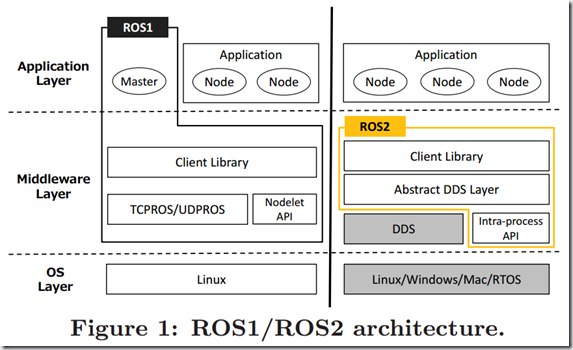
\includegraphics[width=\linewidth]{ros1_ros2_architecture.png}
  \caption{ROS1/ROS2 Architecture \cite{c1}} 
  \label{fig:ros2_architecture}
\end{figure}

ROS1 uses TCP (Transmission Control Protocol) as its communication protocol. TCP is a connection oriented network, this means that TCP tracks all data sent, requiring acknowledgment for each octet (generally), therefore,  ROS1 has a centralized network configuration which requires a running ROS master to take care of naming and registration services. With the help of the master, ROS nodes could find each other on the network and communicate in a peer-to-peer fashion. In ROS1 setting, all nodes will depend on the central ROS master. When the network becomes lossy and unstable(especially if nodes are distributed on several computers), the communication will not be reliable for real-time applications or multi-robot systems.

ROS2 uses Data Distribution Service (DDS) as the communication middleware. UDP is a Data-Centric-Publish-Subscribe(DCPS) model, and this model will create global data space for individual applications to exchange information. DDS will identify a data object by its topic name and then subscribe to this topic, therefore, DDS does not have a central distributor for all information. The DDS publish-subscribe model avoids complex network programming for distributed applications.  ROS2 provides an abstraction layer of DDS, so users do not need to pay attention to the underlying DDS structure. The ROS2 Middleware Interface(RMW) allows users to choose different Quality of Service(QoS). The real-time publish-subscribe (RTPS) protocol allows ROS2 nodes to automatically find each other on the network, thus there is no need for a ROS2 master. This is an important point in terms of fault tolerance.
%%%%%%%%%%%%%%%%%%%%%%%%%%%%%%%%%%%%%%%%%%%%%%%%%%%%%%%%%%%%%%%%%%%%%%%%%%%%%%%%
\section{Related Work}
When ROS2 Bouncy was released, a TurtleBot 2 demo was provided to demonstrate the some popular mapping and localization packages that runs in ROS 2. TurtleBot 2 demo uses Google Cartographer to get maps of the environment, and use AMCL package to localize. TurtleBot 2 demo also provided TurtleBot 2 driver and the Orbbec Astra depth camera sensor driver. At the time this demo was created, ROS2 navigation stack was still under development, therefore, TurtleBot 2 demo uses joystick to manually operate the robot to create maps. 
%%%%%%%%%%%%%%%%%%%%%%%%%%%%%%%%%%%%%%%%%%%%%%%%%%%%%%%%%%%%%%%%%%%%%%%%%%%%%%%%
\section{Method}
The objective of this demo is to build a kobuki SLAM and navigation demo on top of the existing TurtleBot 2 demo, and update packages so that the kobuki robot can achieve SLAM and autonomous navigation using the latest ROS 2 Dashing Diademata release. 
 
\begin{figure}[ht]
  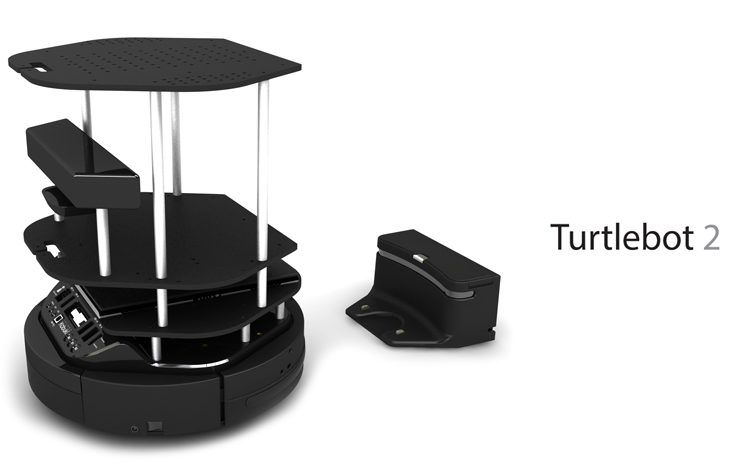
\includegraphics[width=\linewidth]{kobuki_image.jpg}
  \caption{Image of Kobuki Robot(TODO)} 
  \label{fig:Kobuki_image}
\end{figure}
%%%%%%%%%%%%%
\subsection{Hardware and software setup}
\begin{itemize}
\item  Hardware setup 
    \begin{itemize}
        \item Robot: Kobuki (turtlebot2)
        \item Sensor: hokuyo laser scanner
    \end{itemize}{}
\end{itemize}

\begin{itemize}
\item ROS2 Packages:
    \begin{itemize}
        \item Mapping   
            \begin{itemize}
                \item cartographer (binary release available)
                \item cartographer-ros 
            \end{itemize}{}
    \end{itemize}{}
    \begin{itemize}
        \item Visualization
            \begin{itemize}
                \item ros1\_bridge (binary release available)
                \item rviz
            \end{itemize}{}
   
        \item Controller and drivers:
            \begin{itemize}
                \item teleop\_twist\_keyboard (binary release available)
                \item urg\_node: URG laser scan driver 
                \item tutlebot2\_drivers: provide kobuki\_node to drive the Kobuki Robot
            \end{itemize}{}
        \item Simulation:
            \begin{itemize}
                \item Gazebo9 simulation (binary release available)
            \end{itemize}{}
    \end{itemize}{} 
\end{itemize}{}

\begin{itemize}
    \item Simulation Plan (TODO)
        \begin{itemize}
            \item Setup gazebo for kobuki
            \item Setup laser scan
            \item Run cartographer in simulation 
            \item After getting map, try the navigation stack
        \end{itemize}{}
\end{itemize}{}

%%%%%%%%%%%%%
\subsection{Implementation}

% 1. Change CmakeList.txt and package.xml
% 2. Build all packages using colcon build 
% 3. Manually control robot and use Goolge Cartographer to get the map 
% 4. Visualization using ros1_bridge 
1. \textit{Setup Build files} \par \vspace{5pt}
 ROS2 uses a build system called Ament Build tool. Ament is an evolution of catkin that automatically build a set of independent packages base on their dependency topological order. Ament will also install and configure the environment for packages, so the user does not need to follow a specific dependency order to build packages. The package.xml will provide meta information about the packages and their dependencies, and the build configuration are stored in the CMakeList.txt  \par \vspace{5pt}
 
2. \textit{Build packages using colcon build}\par\vspace{5pt}
ROS1 has multiple different building tools such as catkin\_make, catkin\_make\_isolated and catkin\_tools. ROS 2 provides a universal build tool called colcon. This colcon tool makes the building testing and using multiple packages easy. \par\vspace{5pt}

3. \textit{Manual mapping using Cartographer}\par\vspace{5pt}
% launch system 
This demo uses teleop-keyboard to manually operate the Kobuki robot. The cartographer node utilizes the laser scan data obtained from the hokuyo laser scanner and the optometry information published though the kobuki\_node robot driver and create a 2D map. 
This demo uses teleo-keyboard to operate the Kobuki robot, and obtain a map using google cartographer. The rqt\_graph is show in figure \ref{fig:rqt}\par\vspace{5pt}
\begin{figure}[ht]
  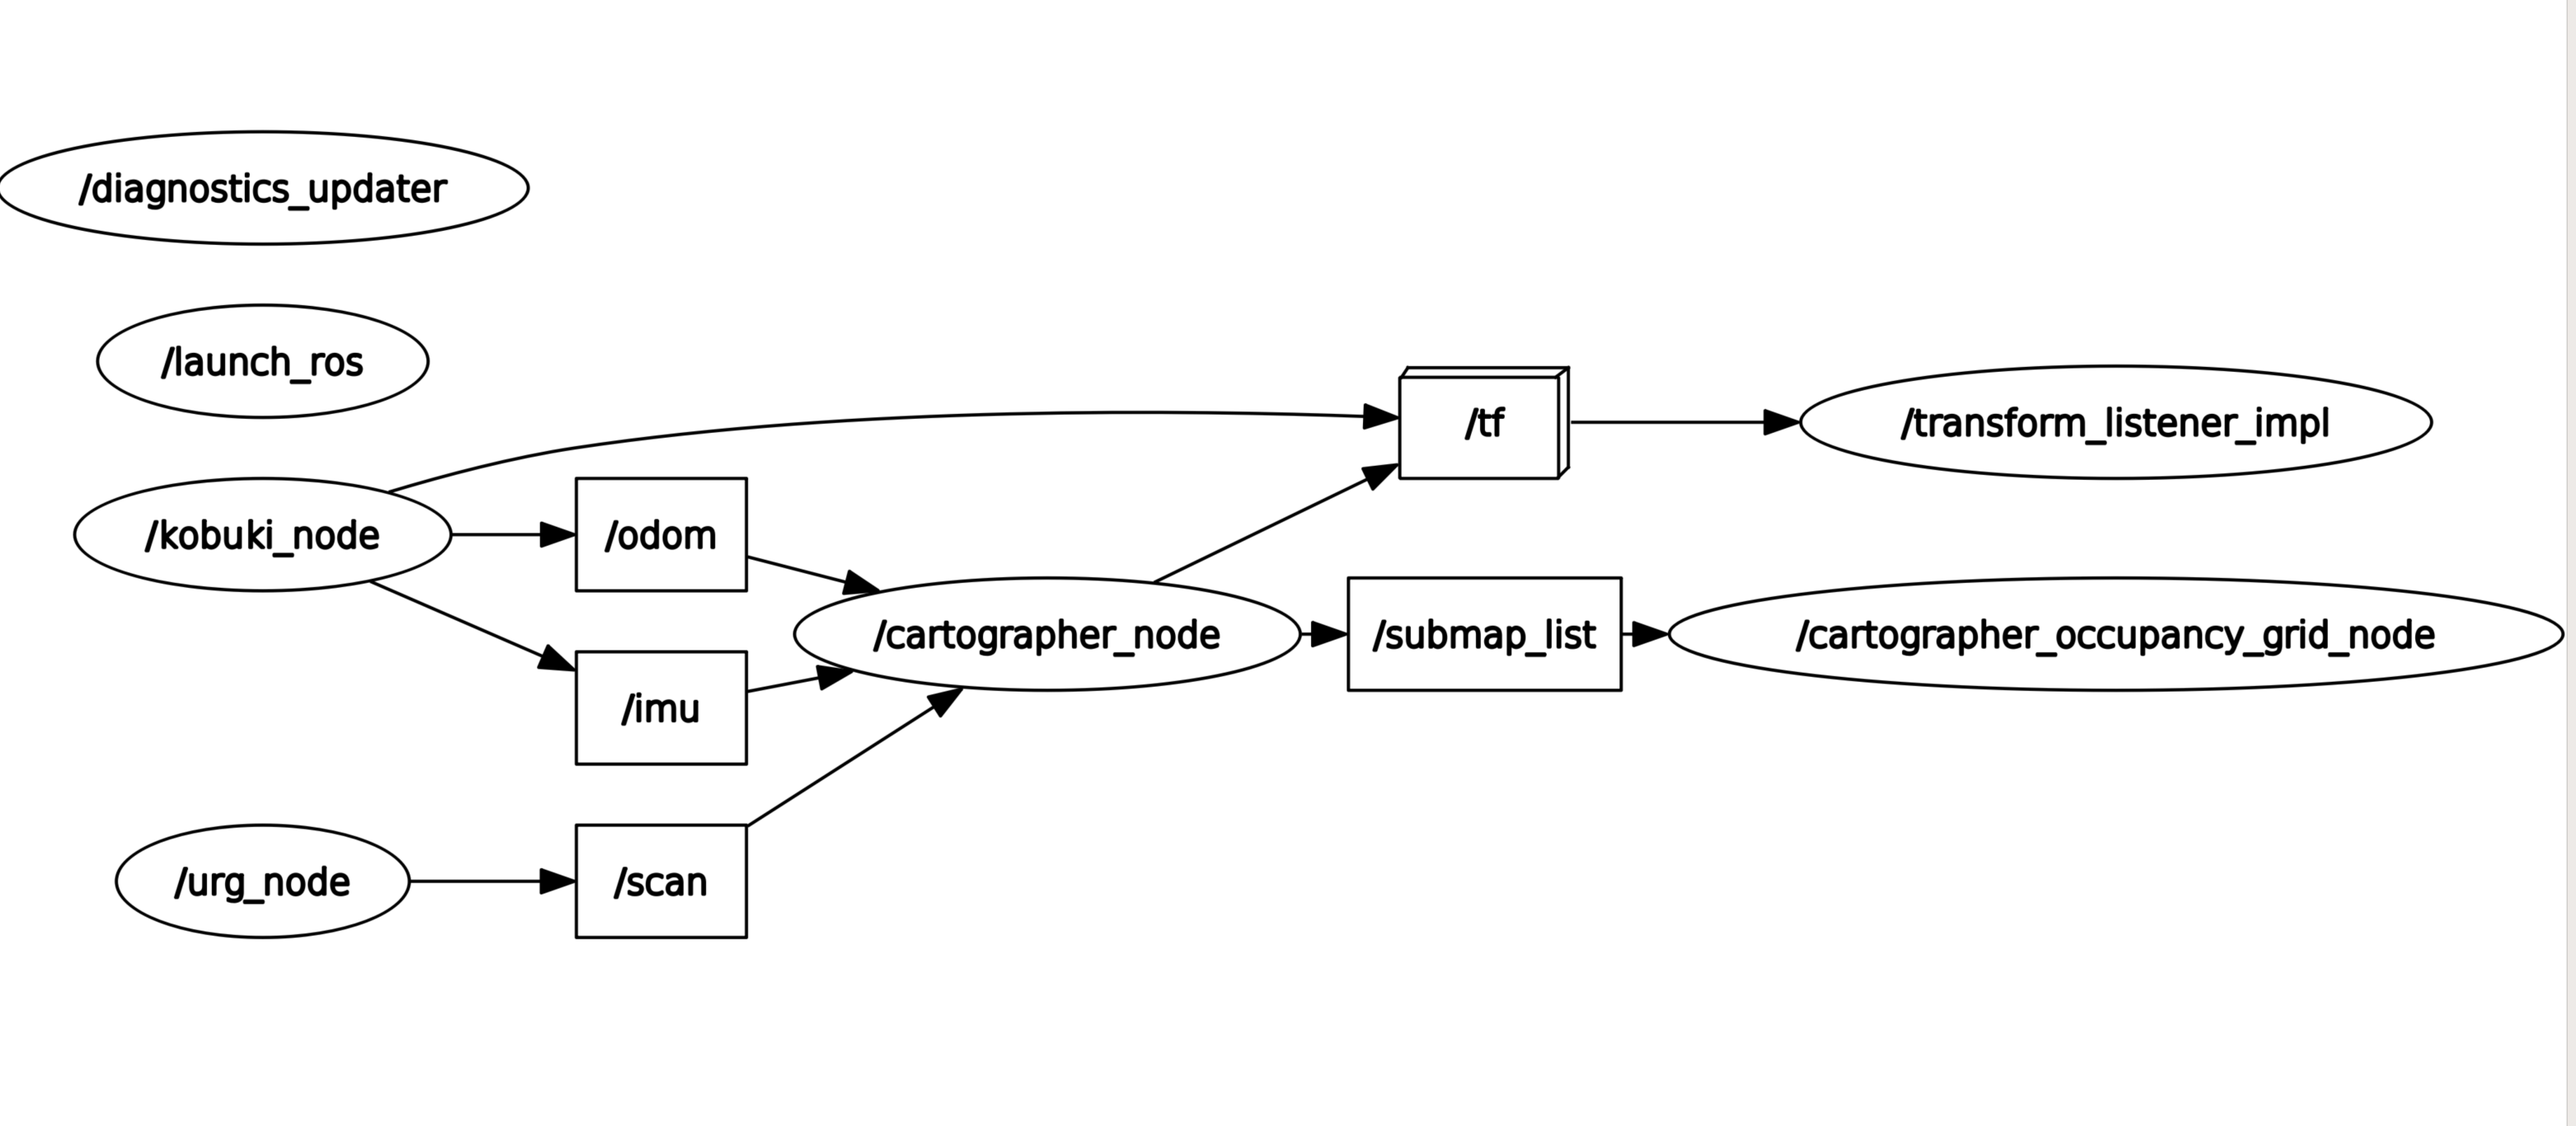
\includegraphics[width=\linewidth]{qrt_graph.png}
  \caption{ROS2 rqt\_graph} 
  \label{fig:rqt}
\end{figure}
4.\textit{Data visualization using ros1\_bridge}\par\vspace{5pt} 
Due to the unstable behavior of rviz2 provided in ROS 2, this demo uses ros1\_bridge to pass data into ROS1 to visualize the map obtained by cartographer. ros1\_bridge provides a network bridge which enables the exchange of messages between ROS 1 and ROS 2. This bridge will establish connection when matching publisher-subscriber pairs are active to a topic on either side of the bridge\cite{c4}. The current version supports most of the common message types in ROS 1 and ROS 2, user can also create their own customized message pairs through a package mapping rule file that matches all messages with the same names and fields within a pair of packages.\par\vspace{5pt} 

5. \textit{Simulation Setup} 
TODO

%%%%%%%%%%%%%%%%%%%%%%%%%%%%%%%%%%%%%%%%%%%%%%%%%%%%%%%%%%%%%%%%%%%%%%%%%%%%%%%%
\section{Results}\label{results}
\subsection{Robot Mapping}
The map shown in figure \ref{fig:map} was obtained by driving the robot in a room. The result draws reasonable boundaries. However area that near large windows shows a large amount of noise due to laser reflection. 
\begin{figure}[ht]
  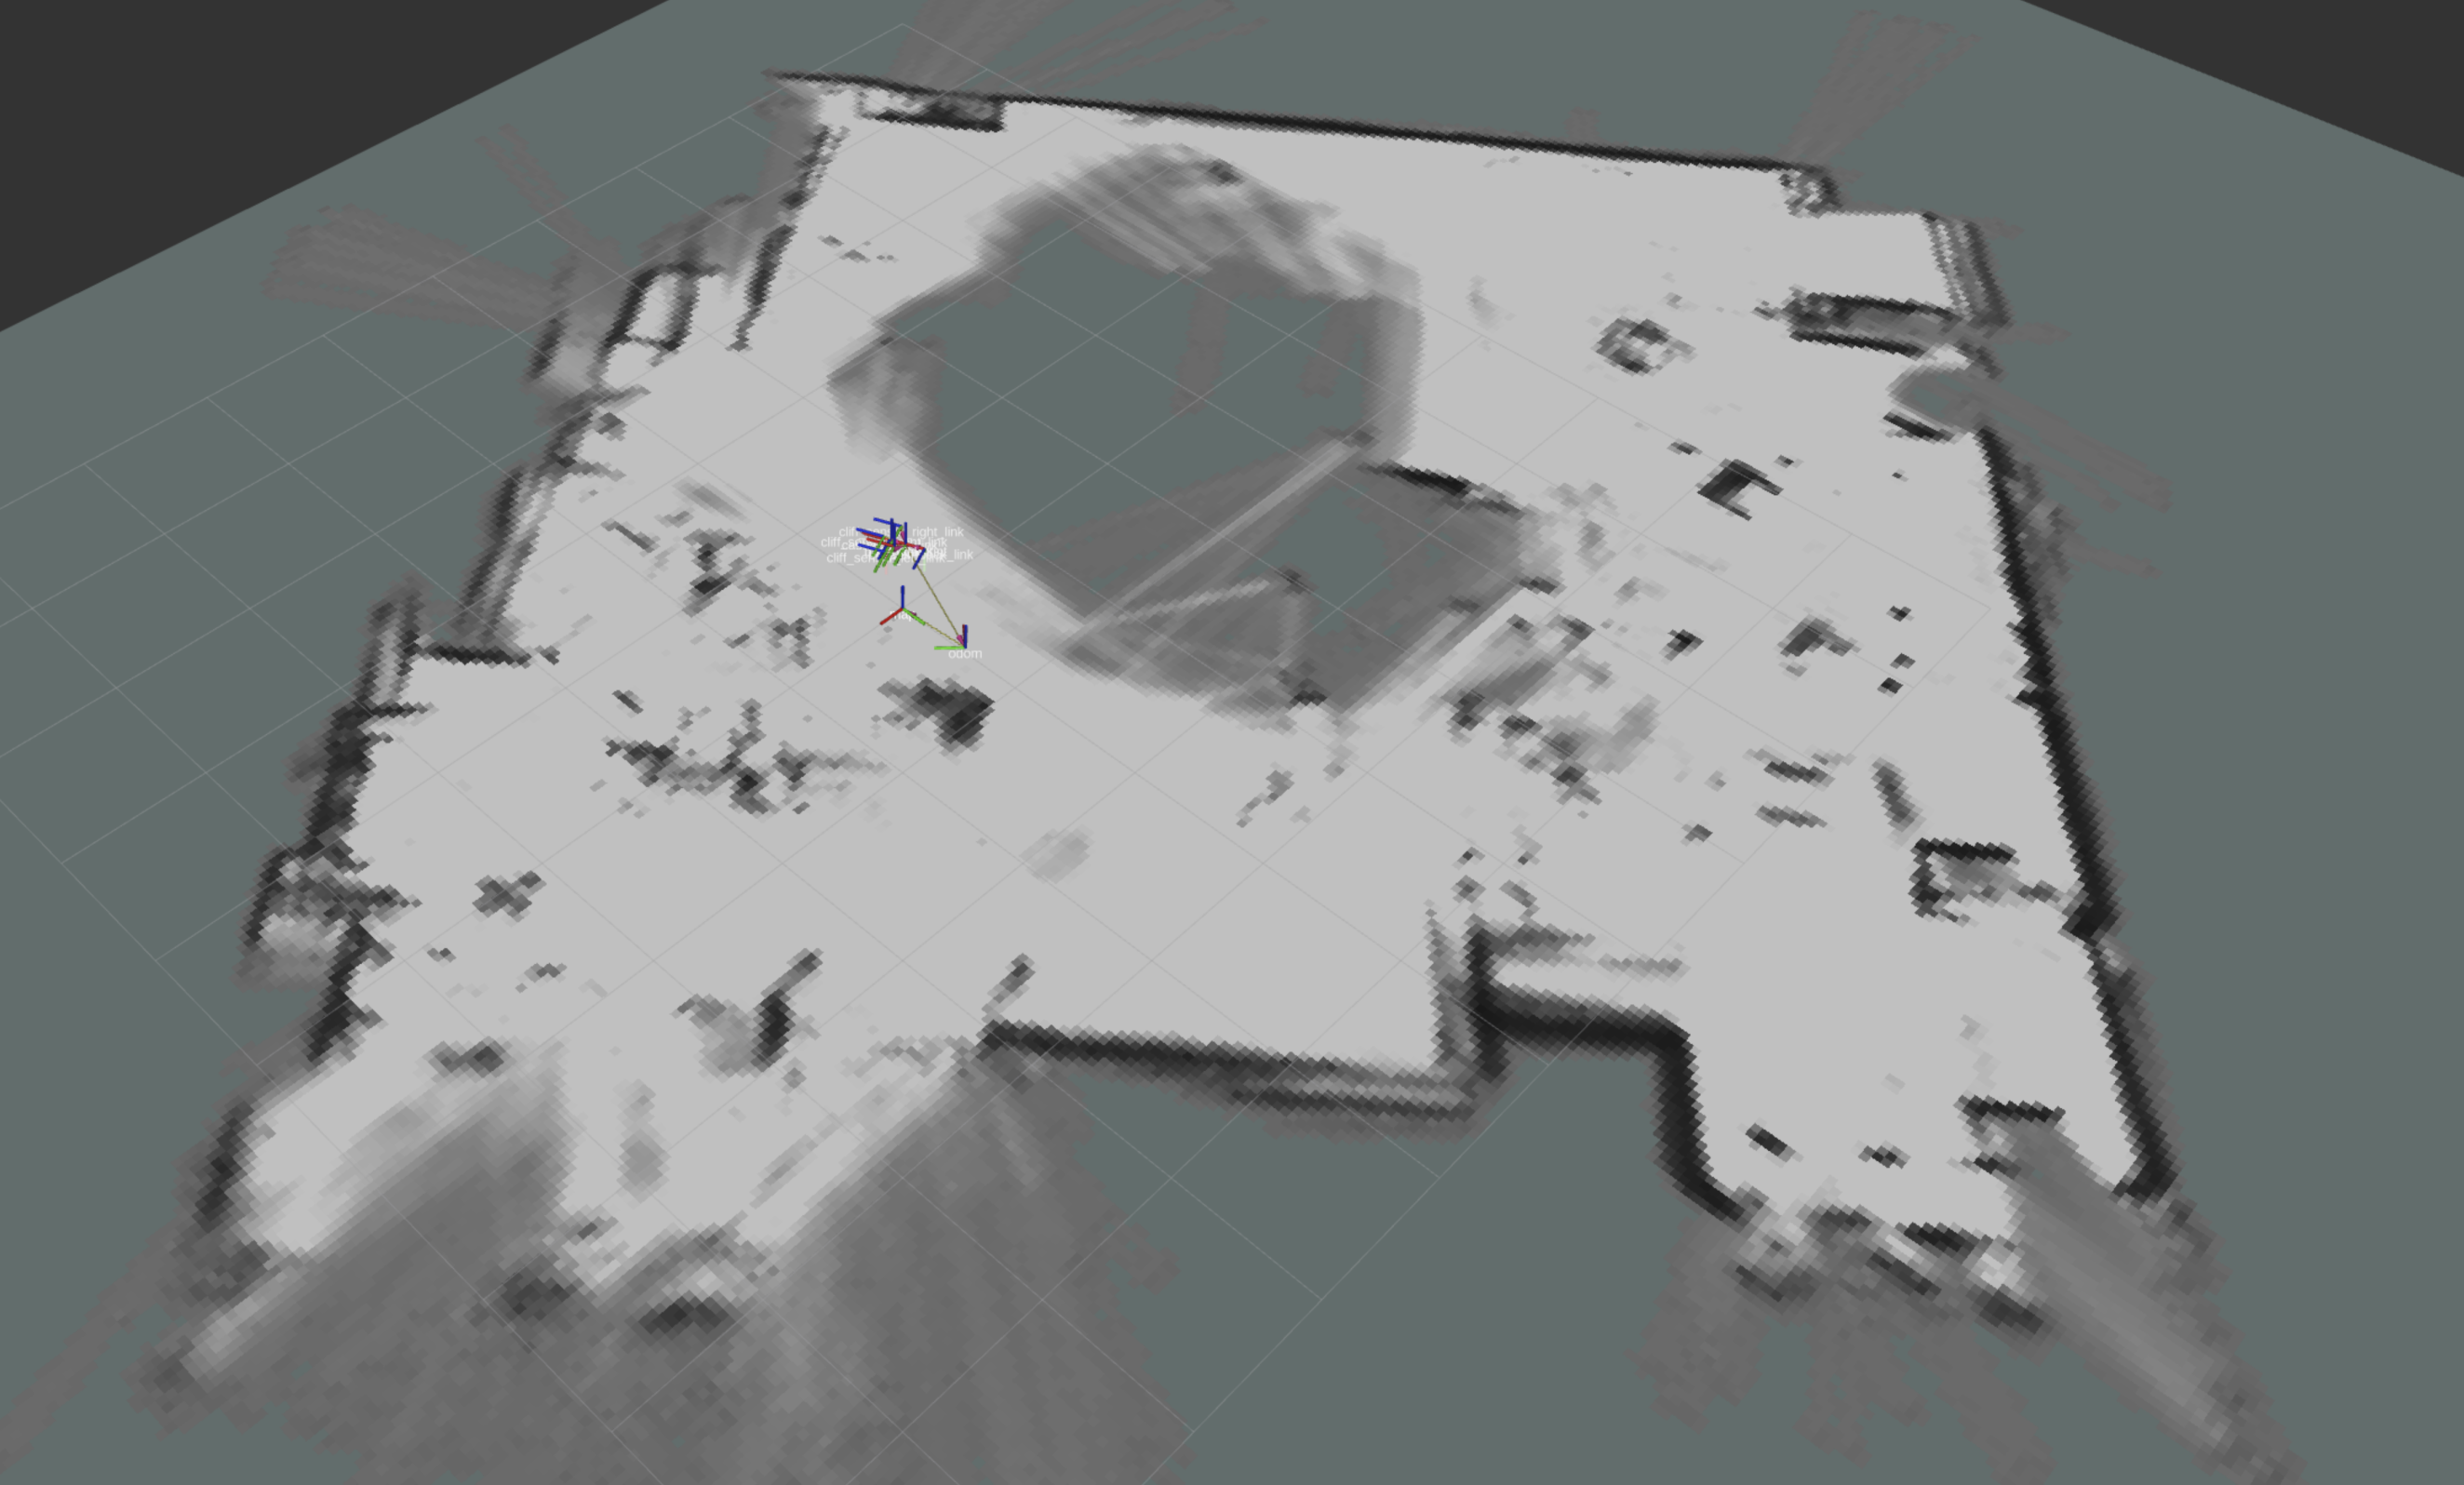
\includegraphics[width=\linewidth]{map.png}
  \caption{map obtained by google cartographer} 
  \label{fig:map}
\end{figure}
\subsection{Gazebo 9 Simulation}
\begin{figure}[ht]
  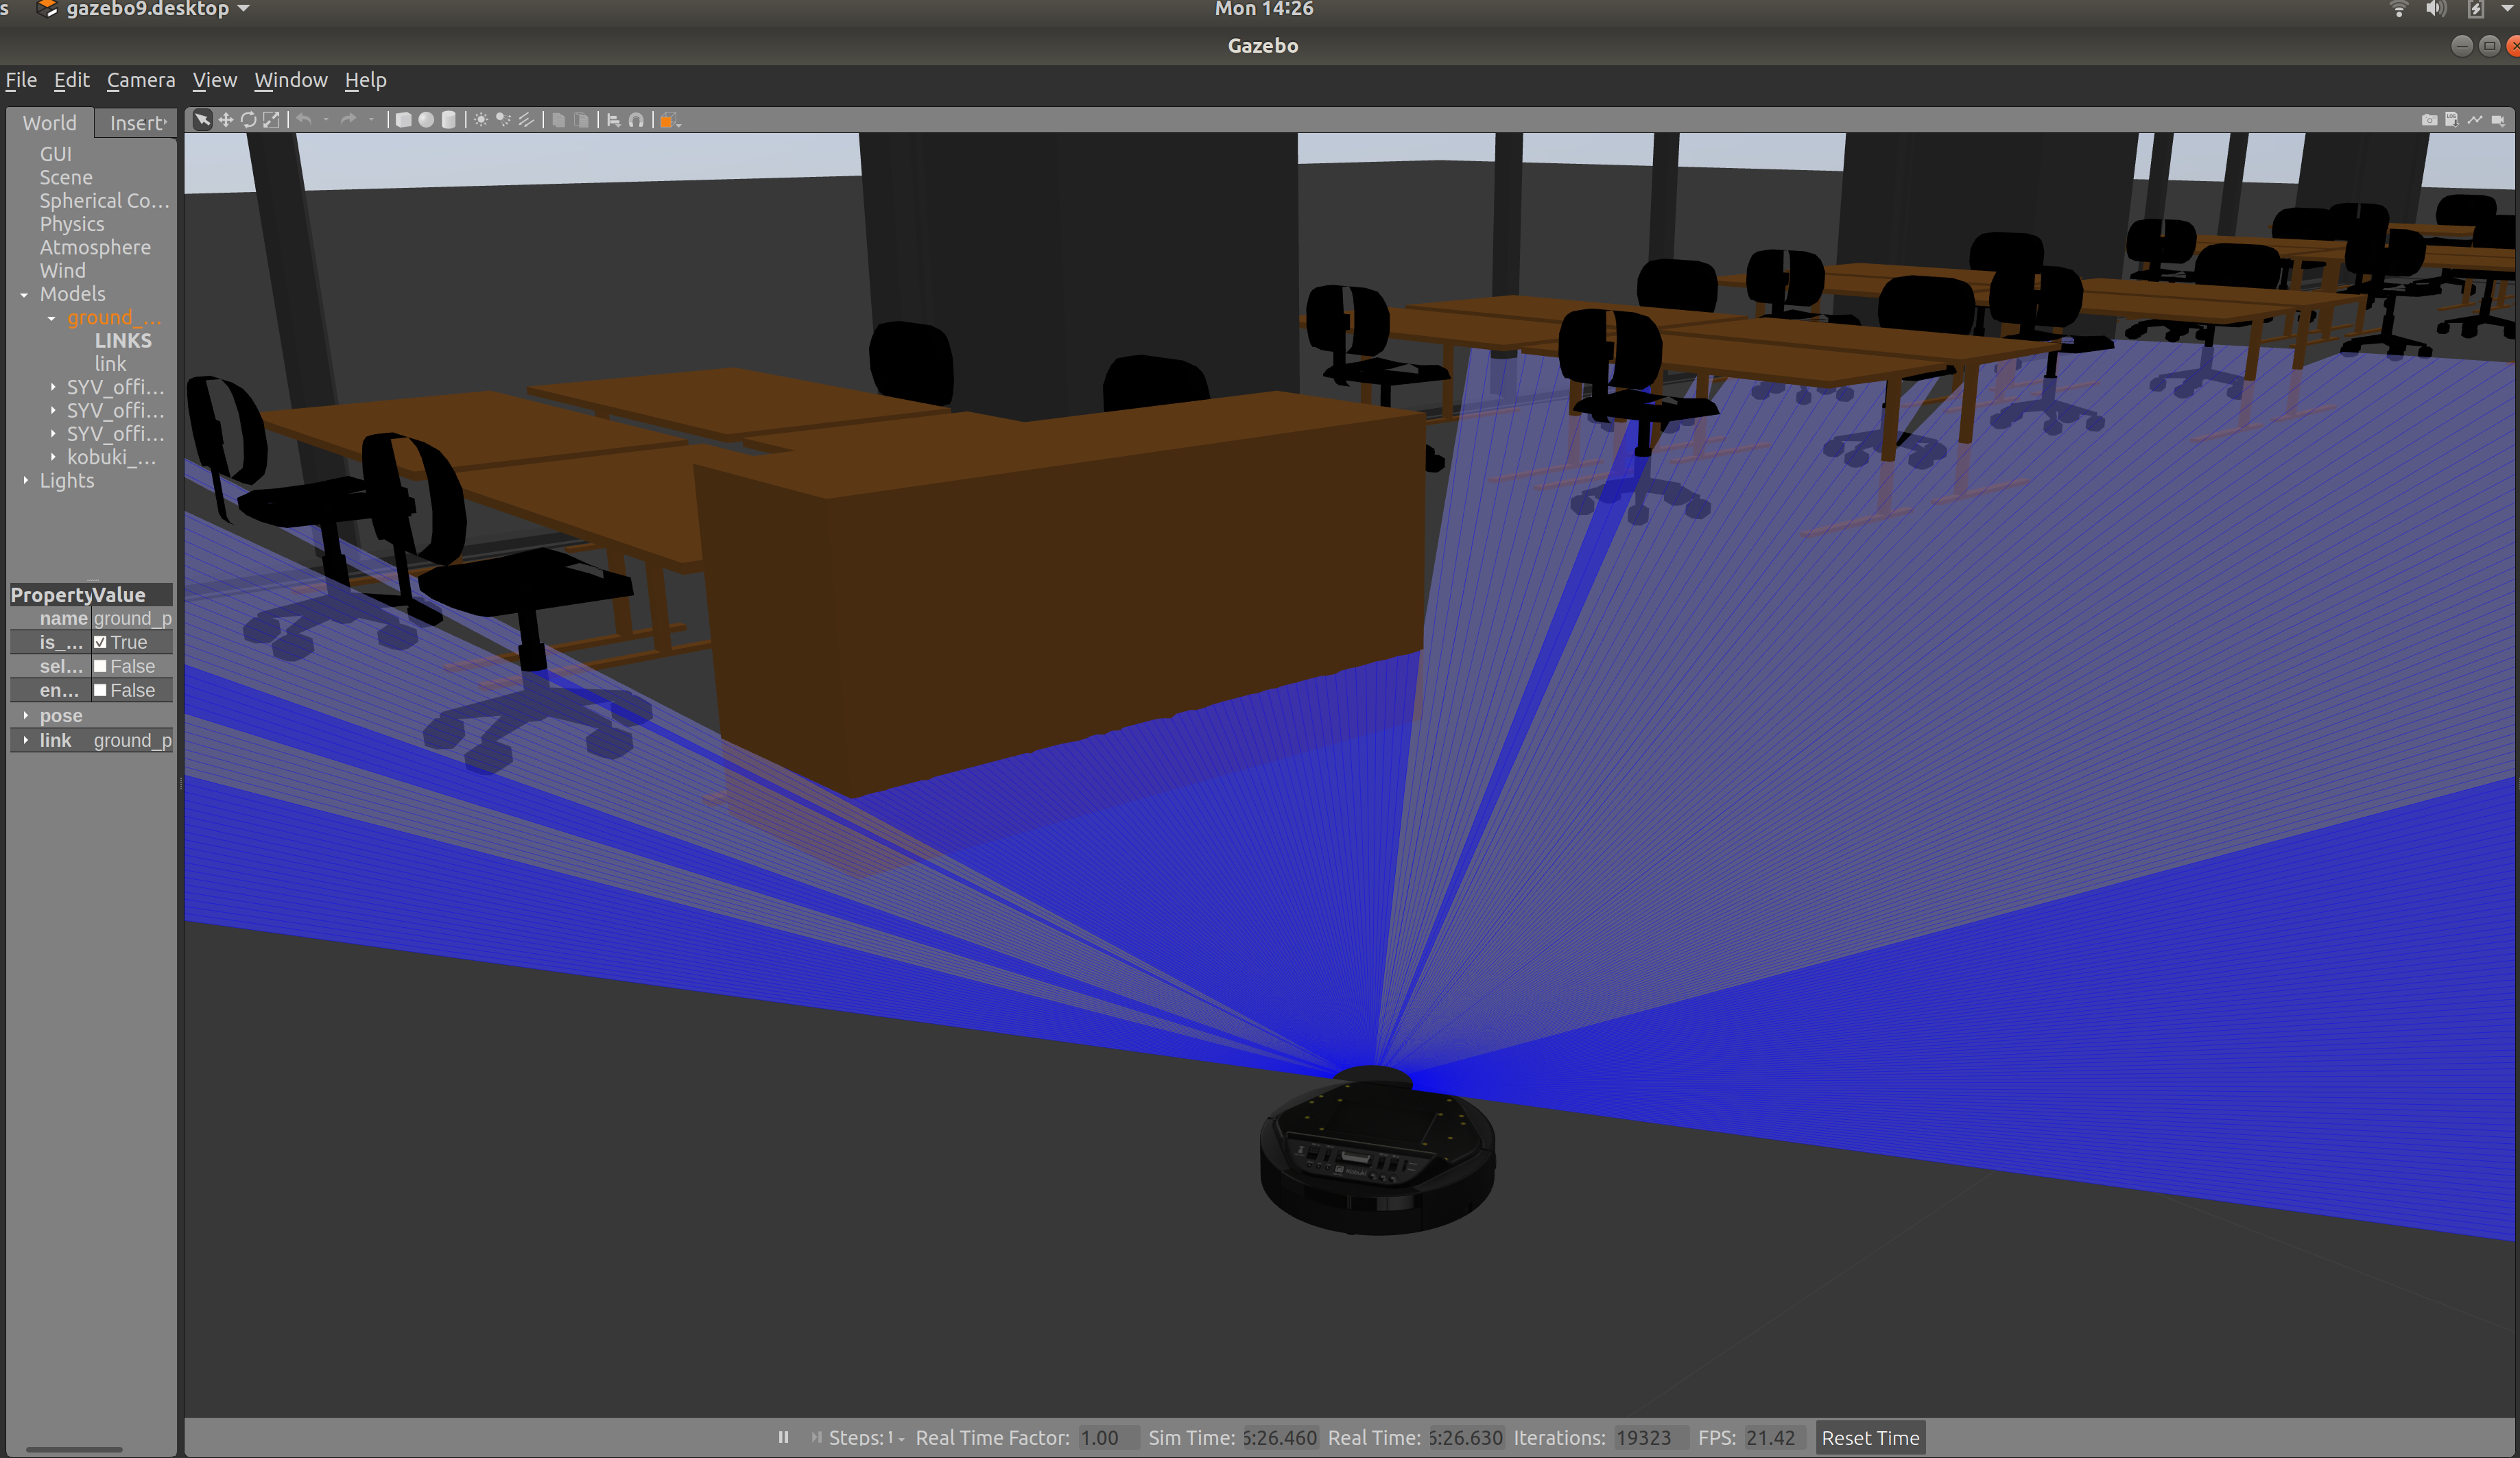
\includegraphics[width=\linewidth]{gazebo_simulation.png}
  \caption{Kobuki and laser scanner in Gazebo 9 Simulation } 
  \label{fig:gazebo}
\end{figure}
%%%%%%%%%%%%%%%%%%%%%%%%%%%%%%%%%%%%%%%%%%%%%%%%%%%%%%%%%%%%%%%%%%%%%%%%%%%%%%%%
\section{Conclusions}\label{conclusions}

%%%%%%%%%%%%%%%%%%%%%%%%%%%%%%%%%%%%%%%%%%%%%%%%%%%%%%%%%%%%%%%%%%%%%%%%%%%%%%%%
\section{Reference}\label{reference}
\addtolength{\textheight}{-12cm}   % This command serves to balance the column lengths
                                  % on the last page of the document manually. It shortens
                                  % the textheight of the last page by a suitable amount.
                                  % This command does not take effect until the next page
                                  % so it should come on the page before the last. Make
                                  % sure that you do not shorten the textheight too much.
%%%%%%%%%%%%%%%%%%%%%%%%%%%%%%%%%%%%%%%%%%%%%%%%%%%%%%%%%%%%%%%%%%%%%%%%%%%%%%%%
\section*{APPENDIX}

%%%%%%%%%%%%%%%%%%%%%%%%%%%%%%%%%%%%%%%%%%%%%%%%%%%%%%%%%%%%%%%%%%%%%%%%%%%%%%%%
\section*{ACKNOWLEDGMENT}
%%%%%%%%%%%%%%%%%%%%%%%%%%%%%%%%%%%%%%%%%%%%%%%%%%%%%%%%%%%%%%%%%%%%%%%%%%%%%%%%
\begin{thebibliography}{99}

\bibitem{c1} Y. Maruyama, S. Kato, and T. Azumi, “Exploring the performance of ROS2,” Proceedings of the 13th International Conference on Embedded Software - EMSOFT 16, 2016. 
\bibitem{c2} Open Source Robotics Foundation(OSRF) http://www.osrfoundation.org/.
\bibitem{c3} Gerkey, B. (2019). Why ROS 2?. [online] Design.ros2.org. Available at: https://design.ros2.org/articles/why\_ros2.html [Accessed 9 Jul. 2019].
\bibitem{c4} GitHub. (2019). ros2/ros1\_bridge. [online] Available at: https://github.com/ros2/ros1\_bridge [Accessed 9 Jul. 2019].
\end{thebibliography}
\end{document}
